\Chapter{\readyforreadingmod{Reification by Parametricity: Fast Setup for Proof by Reflection, in Two Lines of \Ltac}{intro and conclusion being removed / reflowed}}\label{ch:reification-by-parametricity}
\todo{include the trick from https://github.com/coq/coq/issues/5996\#issuecomment-670955273}
\begin{abstract}
  We present a new strategy for performing reification in Coq.
  That is, we show how to generate first-class abstract syntax trees from ``native'' terms of Coq's logic, suitable as inputs to verified compilers or procedures in the \emph{proof-by-reflection} style.
  Our new strategy, based on simple generalization of subterms as variables, is straightforward, short, and fast.
  In its pure form, it is only complete for constants and function applications, but ``let'' binders, eliminators, lambdas, and quantifiers can be accommodated through lightweight coding conventions or preprocessing.

  We survey the existing methods of reification across multiple Coq metaprogramming facilities, describing various design choices and tricks that can be used to speed them up, as well as various limitations.
  We report benchmarking results for 18 variants, in addition to our own, finding that our own reification outperforms 16 of these methods in all cases, and one additional method in some cases; writing an OCaml plugin is the only method tested to be faster.
  Our method is the most concise of the strategies we considered, reifying terms using only two to four lines of \Ltac---beyond lists of the identifiers to reify and their reified variants.
  Additionally, our strategy automatically provides error messages that are no less helpful than Coq's own error messages.
\end{abstract}

\setlength{\belowdisplayskip}{5pt}% \setlength{\belowdisplayshortskip}{0pt}%
\setlength{\abovedisplayskip}{5pt}% \setlength{\abovedisplayshortskip}{0pt}%

\section{Introduction} \label{sec:reification-by-parametricity:intro}

Proof by reflection~\cite{ReflectionTACS97} is an established method for employing verified proof procedures, within larger proofs.
There are a number of benefits to using verified functional programs written in the proof assistant's logic, instead of tactic scripts.
We can often prove that procedures always terminate without attempting fallacious proof steps, and perhaps we can even prove that a procedure gives logically complete answers, for instance telling us definitively whether a proposition is true or false.
In contrast, tactic-based procedures may encounter runtime errors or loop forever.
As a consequence, those procedures must output proof terms, justifying their decisions, and these terms can grow large, making for slower proving and requiring transmission of large proof terms to be checked slowly by others.
A verified procedure need not generate a certificate for each invocation.

The starting point for proof by reflection is \emph{reification}: translating a ``native'' term of the logic into an explicit abstract syntax tree.
We may then feed that tree to verified procedures or any other functional programs in the logic.
The benefits listed above are particularly appealing in domains where goals are very large.
For instance, consider verification of large software systems, where we might want to reify thousands of lines of source code.
Popular methods turn out to be surprisingly slow, often to the point where, counter-intuitively, the majority of proof-execution time is spent in reification -- unless the proof engineer invests in writing a plugin directly in the proof assistant's metalanguage (e.g., OCaml for Coq).

In this paper, we show that reification can be both simpler and faster than with standard methods.
Perhaps surprisingly, we demonstrate how to reify terms almost entirely through reduction in the logic, with a small amount of tactic code for setup and no ML programming.
Though our techniques should be broadly applicable, especially in proof assistants based on type theory, our experience is with Coq, and we review the requisite background in the remainder of this introduction.
In \autoref{sec:reif-survey}, we summarize our survey into prior approaches to reification and provide high-quality implementations and documentation for them, serving a tutorial function independent of our new contributions.
Experts on the subject might want to skip directly to \autoref{sec:reification-by-parametricity}, which explains our alternative technique.
We benchmark our approach against 18 competitors in \autoref{sec:perf}.

\subsection{Proof-Script Primer}
Basic Coq proofs are often written as lists of steps such as \texttt{induction} on some structure, \texttt{rewrite} using a known equivalence, or \texttt{unfold} of a definition.
Very quickly, proofs can become long and tedious, both to write and to read, and hence Coq provides \Ltac, a scripting language for proofs.
As theorems and proofs grow in complexity, users frequently run into performance and maintainability issues with \Ltac.
Consider the case where we want to prove that a large algebraic expression, involving many \letindots\space expressions, is even:
\begin{verbatim}
Inductive is_even : nat -> Prop :=
| even_O : is_even O
| even_SS : forall x, is_even x -> is_even (S (S x)).
Goal is_even (let x := 100 * 100 * 100 * 100 in
              let y := x * x * x * x in
              y * y * y * y).
\end{verbatim}
Coq stack-overflows if we try to reduce this goal.
As a workaround, we might write a lemma that talks about evenness of \letindots, plus one about evenness of multiplication, and we might then write a tactic that composes such lemmas.

Even on smaller terms, though, proof size can quickly become an issue.
If we give a naive proof that 7000 is even, the proof term will contain all of the even numbers between 0 and 7000, giving a proof-term-size blow-up at least quadratic in size (recalling that natural numbers are represented in unary; the challenges remain for more efficient base encodings).
Clever readers will notice that Coq could share subterms in the proof tree, recovering a term that is linear in the size of the goal.
However, such sharing would have to be preserved very carefully, to prevent size blow-up from unexpected loss of sharing, and today's Coq version does not do that sharing.
Even if it did, tactics that rely on assumptions about Coq's sharing strategy become harder to debug, rather than easier.

\subsection{Reflective-Automation Primer}\label{sec:evenness}
Enter reflective automation, which simultaneously solves both the problem of performance and the problem of debuggability.
Proof terms, in a sense, are traces of a proof script.
They provide Coq's kernel with a term that it can check to verify that no illegal steps were taken.
Listing every step results in large traces.

\begin{wrapfigure}[9]{r}{5cm}
%\vspace{-33pt}
\begin{verbatim}
Fixpoint check_is_even
   (n : nat) : bool
  := match n with
     | 0 => true
     | 1 => false
     | S (S n)
       => check_is_even n
     end.
\end{verbatim}
%\vspace{-18pt}
\caption{Evenness Checking}\label{fig:check-is-even}
\end{wrapfigure}
The idea of reflective automation is that, if we can get a formal encoding of our goal, plus an algorithm to \emph{check} the property we care about, then we can do much better than storing the entire trace of the program.
We can prove that our checker is correct once and for all, removing the need to trace its steps.

A simple evenness checker can just operate on the unary encoding of natural numbers (\autoref{fig:check-is-even}).
We can use its correctness theorem to prove goals much more quickly:
\begin{verbatim}
Theorem soundness : forall n, check_is_even n = true -> is_even n.
Goal is_even 2000.
  Time repeat (apply even_SS || apply even_O). (* 1.8 s *)
  Undo.
  Time apply soundness; vm_compute; reflexivity. (* 0.004 s *)
\end{verbatim}
The tactic \texttt{vm\_compute} tells Coq to use its virtual machine for reduction, to compute the value of \texttt{check\_is\_even 2000}, after which \texttt{reflexivity} proves that \texttt{true = true}.
Note how much faster this method is.
In fact, even the asymptotic complexity is better; this new algorithm is linear rather than quadratic in \texttt{n}.

However, even this procedure takes a bit over three minutes to prove \texttt{is\_even (10 * 10 * 10 * 10 * 10 * 10 * 10 * 10 * 10)}.
To do better, we need a formal representation of terms or expressions.

\subsection{Reflective-Syntax Primer}
Sometimes, to achieve faster proofs, we must be able to tell, for example, whether we got a term by multiplication or by addition, and not merely whether its normal form is 0 or a successor.%
%\footnote{%
%  Sometimes this distinction is necessary for generating a proof at all, as is the case in \texttt{nsatz} and \texttt{romega}; there is no way to prove that addition is commutative if you cannot identify what things you were adding in the first place.%
%}

\begin{wrapfigure}[4]{r}{5cm}
%\vspace{-45pt}
\begin{verbatim}
Inductive expr :=
| NatO : expr
| NatS (x : expr) : expr
| NatMul (x y : expr) : expr.
\end{verbatim}
%\vspace{-15pt}
\caption{Simple Expressions}\label{fig:inductive-expr-no-letin}
\end{wrapfigure}

A reflective automation procedure generally has two steps.
The first step is to \emph{reify} the goal into some abstract syntactic representation, which we call the \emph{term language} or an \emph{expression language}.
The second step is to run the algorithm on the reified syntax.

What should our expression language include?
At a bare minimum, we must have multiplication nodes, and we must have \texttt{nat} literals.
If we encode \texttt{S} and \texttt{O} separately, a decision that will become important later in~\autoref{sec:reification-by-parametricity}, we get the inductive type of \autoref{fig:inductive-expr-no-letin}.

Before diving into methods of reification, let us write the evenness checker.
\begin{verbatim}
Fixpoint check_is_even_expr (t : expr) : bool
  := match t with
     | NatO => true
     | NatS x => negb (check_is_even_expr x)
     | NatMul x y => orb (check_is_even_expr x) (check_is_even_expr y)
     end.
\end{verbatim}
%We have used \texttt{negb} and \texttt{orb} from the standard library for boolean negation and disjunction respectively.

Before we can state the soundness theorem (whenever this checker returns \texttt{true}, the represented number is even), we must write the function that tells us what number our expression represents, called \emph{denotation} or \emph{interpretation}:
\begin{verbatim}
Fixpoint denote (t : expr) : nat
  := match t with
     | NatO => O
     | NatS x => S (denote x)
     | NatMul x y => denote x * denote y
     end.

Theorem check_is_even_expr_sound (e : expr)
  : check_is_even_expr e = true -> is_even (denote e).
\end{verbatim}

Given a tactic \texttt{Reify} to produce a reified term from a \verb|nat|, we can time \verb|check_is_even_expr|.
It is instant on the last example.%, \texttt{10 * 10 * 10 * 10 * 10 * 10 * 10 * 10 * 10}.

Before we proceed to reification, we will introduce one more complexity.
If we want to support our initial example with \letindots\space efficiently, we must also have \texttt{let}-expressions.
Our current procedure that inlines \texttt{let}-expressions takes 19 seconds, for example, on \texttt{let x0 := 10 * 10 in let x1 := x0 * x0 in \ldots\space let x24 := x23 * x23 in x24}.
The choices of representation include higher-order abstract syntax (HOAS)~\cite{HOAS}, parametric higher-order abstract syntax (PHOAS)~\cite{PhoasICFP08}, and de Bruijn indices~\cite{debruijn1972}.
The PHOAS representation is particularly convenient.
In PHOAS, expression binders are represented by binders in Gallina, the functional language of Coq, and the expression language is parameterized over the type of the binder.
%We make this binder type implicit so that we can often omit writing it.
Let us define a constant and notation for \texttt{let} expressions as definitions (a common choice in real Coq developments, to block Coq's default behavior of inlining \texttt{let} binders silently; the same choice will also turn out to be useful for reification later).
We thus have: \label{sec:phoas-expr-def}
\begin{verbatim}
Inductive expr {var : Type} :=
| NatO : expr
| NatS : expr -> expr
| NatMul : expr -> expr -> expr
| Var : var -> expr
| LetIn : expr -> (var -> expr) -> expr.
Definition Let_In {A B} (v : A) (f : A -> B) := let x := v in f x.
Notation "'dlet' x := v 'in' f" := (Let_In v (fun x => f)).
Notation "'elet' x := v 'in' f" := (LetIn v (fun x => f)).
Fixpoint denote (t : @expr nat) : nat
  := match t with
     | NatO => O
     | NatS x => S (denote x)
     | NatMul x y => denote x * denote y
     | Var v => v
     | LetIn v f => dlet x := denote v in denote (f x)
     end.
\end{verbatim}

A full treatment of evenness checking for PHOAS would require proving well-formedness of syntactic expressions; for a more complete discussion of PHOAS, we refer the reader elsewhere~\cite{PhoasICFP08}.
Using \texttt{Wf} to denote the well-formedness predicate, we could prove a theorem
\begin{verbatim}
Theorem check_is_even_expr_sound (e : ∀ var, @expr var) (H : Wf e)
: check_is_even_expr (e bool) = true -> is_even (denote (e nat)).
\end{verbatim}
To complete the picture, we would need a tactic \texttt{Reify} which took in a term of type \texttt{nat} and gave back a term of type \texttt{forall var, @expr var}, plus a tactic \texttt{prove\_wf} which solved a goal of the form \texttt{Wf e} by repeated application of constructors.
Given these, we could solve an evenness goal by writing%
\footnote{%
  Note that for the \texttt{refine} to be fast, we must issue something like \texttt{Strategy -10 [denote]} to tell Coq to unfold \texttt{denote} before \texttt{Let\_In}.
  }
\begin{verbatim}
match goal with
| [ |- is_even ?v ]
  => let e := Reify v in
     refine (check_is_even_expr_sound e _ _);
     [ prove_wf | vm_compute; reflexivity ]
end.
\end{verbatim}
%\todo{Should we mention that for the \texttt{refine} to be fast, we need a \texttt{Strategy} command to tell Coq to unfold \texttt{denote} before \texttt{Let\_In}?}

\section{Methods of Reification} \label{sec:reif-survey}

We implemented reification in 18 different ways, using 6 different metaprogramming facilities in the Coq ecosystem: Ltac, Ltac2, Mtac~\cite{lessadhoc}, type classes~\cite{sozeau2008first}, canonical structures~\cite{gonthier2016small}, and reification-specific OCaml plugins (quote~\cite{quote-plugin}, template-coq~\cite{TemplateCoq}, ours).
\autoref{fig:ltac-reify-nobinders} displays the simplest case: an Ltac script to reify a tree of function applications and constants.
Unfortunately, all methods we surveyed become drastically more complicated or slower (and usually both) when adapted to reify terms with variable bindings such as \texttt{let}-\texttt{in} or \texttt{$\lambda$} nodes.

\begin{wrapfigure}[10]{r}{6.4cm}
%\vspace{-11pt}
\begin{verbatim}
Ltac f v x := (* reify var term *)
  lazymatch x with
  | O => constr:(@NatO v)
  | S ?x => let X := f v x in
            constr:(@NatS v X)
  | ?x*?y => let X := f v x in
             let Y := f v y in
             constr:(@NatMul v X Y)
  end.
\end{verbatim}
%\vspace{-20pt}
\caption{Reification Without Binders in \Ltac}\label{fig:ltac-reify-nobinders}
\end{wrapfigure}

We have made detailed walkthroughs and source code of these implementations available\footnote{\url{https://github.com/mit-plv/reification-by-parametricity}} in hope that they will be useful for others considering implementing reification using one of these metaprogramming mechanisms, instructive as nontrivial examples of multiple metaprogramming facilities, or helpful as a case study in Coq performance engineering.
However, we do \emph{not} recommend reading these out of general interest:
most of the complexity in the described implementations strikes us as needless,
with significant aspects of the design being driven by surprising behaviors, misfeatures, bugs, and performance bottlenecks of the underlying machinery as opposed to the task of reification.

\section{Reification by Parametricity} \label{sec:reification-by-parametricity}

We propose factoring reification into two passes, both of which essentially have robust, built-in implementations in Coq: \emph{abstraction} or \emph{generalization}, and \emph{substitution} or \emph{specialization}.


\begin{wrapfigure}[10]{r}{7cm}
%    \vspace{-40pt}
    \[
    \xymatrix{
        \txt{term}
        \ar@<1ex>[ddr]|{\txt{\rotatebox{-40}{generalize}}}
        \ar@<-1ex>@{-->}[rr]_{\txt{reify}}
        &&
        \txt{reified \\ syntax}
        \ar@<-1ex>[ll]_{\txt{denote}}
        \ar@<-1ex>[ddl]|{\txt{\rotatebox{40}{generalize}}}
        \\ \\
        &
        \txt{abstracted term}
        \ar@<1ex>[uul]|{\txt{\rotatebox{-40}{specialize}}}
        \ar@<-1ex>[uur]|{\txt{\rotatebox{40}{specialize}}}
    }
    \]
%    \vspace{-20pt}
    \caption{Abstraction and Reification}\label{fig:denote-reify}
\end{wrapfigure}

The key insight to this factoring is that the shape of a reified term is essentially the same as the shape of the term that we start with.
We can make precise the way these shapes are the same by abstracting over the parts that are different, obtaining a function that can be specialized to give either the original term or the reified term.

That is, we have the commutative triangle in \autoref{fig:denote-reify}.

\subsection{Case-By-Case Walkthrough} \label{sec:case-by-case-walkthrough}
\subsubsection{Function Applications And Constants.} \label{sec:reification-by-parametricity-diagram}\label{sec:walkthrough-func-const}
Consider the example of reifying $2\times 2$.
In this case, the \emph{term} is $2 \times 2$ or (mul (S (S O)) (S (S O))).

To reify, we first \emph{generalize} or \emph{abstract} the term $2\times 2$ over the successor function S, the zero constructor O, the multiplication function mul, and the type $\mathbb N$ of natural numbers.
We get a function taking one type argument and three value arguments:
$$\Lambda N. \; \lambda (\textsc{Mul} : N \to N \to N) \; (\text{O} : N) \; (\text{S} : N \to N). \; \text{\textsc{Mul} (S (S O)) (S (S O))}$$

We can now specialize this term in one of two ways: we may substitute $\mathbb N$, mul, O, and S, to get back the term we started with; or we may substitute \texttt{expr}, \texttt{NatMul}, \texttt{NatO}, and \texttt{NatS} to get the reified syntax tree
\[
\texttt{NatMul (NatS (NatS NatO)) (NatS (NatS NatO))}
\]

This simple two-step process is the core of our algorithm for reification:
abstract over all identifiers (and key parts of their types) and specialize to syntax-tree constructors for these identifiers.

\subsubsection{Wrapped Primitives: ``Let'' Binders, Eliminators, Quantifiers.}\label{sec:walkthrough-wrapped}

The above procedure can be applied to a term that contains ``let'' binders to get a
PHOAS syntax tree that represents the original term, but doing so would not capture
sharing. The result would contain native ``let'' bindings of subexpressions, not
PHOAS let expressions. Call-by-value evaluation of any procedure applied to the
reification result would first substitute the let-bound subexpressions --
leading to potentially exponential blowup and, in practice, memory exhaustion.

The abstraction mechanisms in all proof assistants (that we know about) only allow abstracting over terms, not language primitives.
However, primitives can often be wrapped in explicit definitions, which we \emph{can} abstract over.
For example, we already used a wrapper for ``let'' binders, and terms that use it can be reified by abstracting over that definition.
If we start with the expression
\[
\text{\texttt{dlet} }a := 1\texttt{ in }a \times a
\]
and abstract over $(\texttt{@Let\_In $\mathbb N$ $\mathbb N$})$, S, O, mul, and $\mathbb{N}$,
we get a function of one type argument and four value arguments:
\begin{multline*}
\Lambda N.\,\lambda
\ (\textsc{Mul} : N \to N \to N).
\ \lambda (\text{O} : N).
\ \lambda (\text{S} : N \to N). \\
\ \lambda (\textsc{LetIn} : N \to (N\to N)\to N).
\ \textsc{LetIn (S O) ($\lambda a.$ Mul $a$ $a$)}
\end{multline*}
We may once again specialize this term to obtain either our original term or the reified syntax.
Note that to obtain reified PHOAS syntax, we must include a \texttt{Var} node in the \texttt{LetIn} expression; we substitute $(\lambda x\ f.\ \texttt{LetIn}\ x\ (\lambda v.\ f\ (\texttt{Var}\ v)))$ for \textsc{LetIn} to obtain the PHOAS syntax tree
\[
  \texttt{LetIn (NatS NatO) ($\lambda v.$ NatMul (Var $v$) (Var $v$))}
\]

Wrapping a metalanguage primitive in a definition in the code to be reified is in general sufficient for reification by parametricity.
Pattern matching and recursion cannot be abstracted over directly, but if the same code is expressed using eliminators, these can be handled like other functions.
Similarly, even though $\forall$/$\Pi$ cannot be abstracted over, proof automation that itself introduces universal quantifiers before reification can easily wrap them in a marker definition (\texttt{\_forall T P := forall (x:T), P x}) that can be.
Existential quantifiers are not primitive in Coq and can be reified directly.

\subsubsection{Lambdas.}\label{sec:walkthrough-lambdas}

While it would be sufficient to require that, in code to be reified, we write all lambdas with a named wrapper function, that would significantly clutter the code.
We can do better by making use of the fact that a PHOAS object-language lambda (\texttt{Abs} node) consists of a metalanguage lambda that binds a value of type \texttt{var}, which can be used in expressions through constructor $\mathtt{Var} : \mathtt{var} \to \mathtt{expr}$.
Naive reification by parametricity would turn a lambda of type $N \to N$ into a lambda of type $\mathtt{expr} \to \mathtt{expr}$.
A reification procedure that explicitly recurses over the metalanguage syntax could just precompose this recursive-call result with \texttt{Var} to get the desired object-language encoding of the lambda, but handling lambdas specially does not fit in the framework of abstraction and specialization.

First, let us handle the common case of lambdas that appear as arguments to higher-order functions.
One easy approach: while the parametricity-based framework does not allow for special-casing lambdas, it is up to us to choose how to handle functions that we expect will take lambdas as arguments.
We may replace each higher-order function with a metalanguage lambda that wraps the higher-order arguments in object-language lambdas, inserting \texttt{Var} nodes as appropriate.
Code calling the function $\text{\texttt{sum\_upto} }n\; f := f(0) + f(1) + \cdots + f(n)$ can be reified by abstracting over relevant definitions and substituting
$(\lambda n\ f.\ \texttt{SumUpTo}\ n\ (\texttt{Abs}\ (\lambda v.\ f\ (\texttt{Var}\ v))))$ for $\text{\texttt{sum\_upto}}$.
Note that the expression plugged in for \texttt{sum\_upto} differs from the one plugged in for \texttt{Let\_In} only in the use of a deeply embedded abstraction node.
If we wanted to reify \texttt{LetIn} as just another higher-order function (as opposed to a distinguished wrapper for a primitive), the code would look identical to that for \texttt{sum\_upto}.

It would be convenient if abstracting and substituting for functions that take higher-order arguments were enough to reify lambdas, but here is a counterexample.
\[
  \lambda\ x\ y.\ x \times ((\lambda\ z.\ z \times z)\ y)
\]
\[
  \Lambda N. \; \lambda (\textsc{Mul} : N \to N \to N).\ \lambda\ (x\ y : N).\ \texttt{Mul}\ x\ ((\lambda\ (z : N).\ \texttt{Mul}\ z\  z)\ y)
\]
\[
  \lambda\ (x\ y : \texttt{expr}).\ \texttt{NatMul}\ x\ (\texttt{NatMul}\ y\  y)
\]
The result is not even a PHOAS expression. We claim a desirable reified form is
\[
  \texttt{Abs}(\lambda\ x.\ \texttt{Abs}(\lambda\ y.\ \texttt{NatMul}\ (\texttt{Var}\ x)\ (\texttt{NatMul}\ (\texttt{Var}\ y)\  (\texttt{Var}\ y))))
\]
Admittedly, even our improved form is not quite precise: $\lambda\ z.\, z \times z$ has been lost. However, as almost all standard Coq tactics silently reduce applications of lambdas, working under the assumption that functions not wrapped in definitions will be arbitrarily evaluated during scripting is already the norm.
Accepting that limitation, it remains to consider possible occurrences of metalanguage lambdas in normal forms of outputs of reification as described so far.
As lambdas in \texttt{expr} nodes that take metalanguage functions as arguments (\texttt{LetIn}, \texttt{Abs}) are handled by the rules for these nodes, the remaining lambdas must be exactly at the head of the expression.
Manipulating these is outside of the power of abstraction and specialization; we recommend postprocessing using a simple recursive tactic script.

\subsection{Commuting Abstraction and Reduction} \label{sec:commute-abstraction-reduction}
Sometimes, the term we want to reify is the result of reducing another term.
For example, we might have a function that reduces to a term with a variable number of \texttt{let} binders.\footnote{%
    More realistically, we might have a function that represents big numbers using multiple words of a user-specified width.
    In this case, we may want to specialize the procedure to a couple of different bitwidths, then reifying the resulting partially reduced term.%
}
We might have an inductive type that counts the number of \letindots\space nodes we want in our output.
\label{sec:count-def}
\begin{verbatim}
Inductive count := none | one_more (how_many : count).
\end{verbatim}
It is important that this type be syntactically distinct from $\mathbb N$ for reasons we will see shortly.

\begin{wrapfigure}[3]{r}{7cm}
%    \vspace{-33pt}
    \[
    \xymatrix@C=1pt{
        \txt{unreduced term \\ (big $1$ $n$)} \ar[d]_{\txt{\\reduce}} \\
        \txt{reduced \\ term}
        \ar@<1ex>[ddr]|{\txt{\rotatebox{-45}{generalize}}}
        \ar@<-1ex>@{-->}[rr]_{\txt{reify}}
        &&
        \txt{reified \\ syntax}
        \ar@<-1ex>[ll]_{\txt{denote}}
        \ar@<-1ex>[ddl]|{\txt{\rotatebox{52}{generalize}}}
        \\ \\
        &
        \txt{abstracted term}
        \ar@<1ex>[uul]|{\txt{\rotatebox{-45}{specialize}}}
        \ar@<-1ex>[uur]|{\txt{\rotatebox{52}{specialize}}}
    }
    \]
%    \vspace{-10pt}
    \caption{Abstraction, Reification, Reduction} \label{fig:reduce-denote-reify}
\end{wrapfigure}

We can then define a recursive function that constructs some number of nested \texttt{let} binders:
\label{sec:big-def}
\begin{verbatim}
Fixpoint big (x:nat) (n:count)
  : nat
  := match n with
     | none => x
     | one_more n'
      => dlet x' := x * x in
         big x' n'
     end.
\end{verbatim}
Our commutative diagram in \autoref{fig:denote-reify} now has an additional node, becoming \autoref{fig:reduce-denote-reify}.
Since generalization and specialization are proportional in speed to the size of the term begin handled, we can gain a significant performance boost by performing generalization before reduction.
To explain why, we split apart the commutative diagram a bit more; in reduction, there is a $\delta$ or unfolding step, followed by a $\beta\iota$ step that reduces applications of $\lambda$s and evaluates recursive calls.
In specialization, there is an application step, where the $\lambda$ is applied to arguments, and a $\beta$-reduction step, where the arguments are substituted.
To obtain reified syntax, we may perform generalization after $\delta$-reduction (before $\beta\iota$-reduction), and we are not required to perform the final $\beta$-reduction step of specialization to get a well-typed term.
It is important that unfolding \texttt{big} results in exposing the body for generalization, which we accomplish in Coq by exposing the anonymous recursive function; in other languages, the result may be a primitive eliminator applied to the body of the fixpoint.
Either way, our commutative diagram thus becomes \label{sec:expanded-reif-diagram}
\[
\xymatrix@R=0.5em{
    \txt{unreduced term} \ar[d]^{\delta} \\
    \txt{small partially \\ reduced term}
    \ar[r]^{\beta\iota}
    \ar@<1ex>[ddddrr]
    & \txt{reduced \\ term}
    \ar@<1ex>[ddr]
    \ar@<-1ex>@{-->}[rr]
    &&
    \txt{reduced \\ reified syntax}
    \ar@<-1ex>[ll]
    \ar@<-1ex>[ddl]
    \\ \\
    &&
    \txt{abstracted \\ term}
    \ar@<1ex>[uul]
    \ar@<-1ex>[uur]%|{\text{application; $\beta$-reduction}}
    &
    \txt{unreduced \\ reified syntax}
    \ar@<1ex>[ddl]
    \ar[uu]_{\beta\iota}
    \\ \\
    &&
    \txt{unreduced \\ abstracted term}
    \ar@<1ex>[uuuull]
    \ar@<1ex>[uur]^{\rotatebox{25}{\llap{\text{application\hspace*{-2em}}}}}
}
\]
%\[
%\xymatrix{
%    \txt{unreduced term} \ar[d]^{\delta} \\
%    \txt{small partially \\ reduced term} \ar[r]^{\beta\iota} \ar@/_1pc/[dd]
%    & \txt{reduced term} \ar@/_1pc/[dd] \\
%    &&& \txt{reduced \\ reified syntax}
%    \\
%    \txt{unreduced \\ abstrated term}\ar[r]^{\beta\iota} \ar@/_1pc/[uu] \ar@/_1.5pc/[dr]_{\text{application}}
%    &\txt{abstracted term} \ar@/_1pc/[uu]
%    \ar@/_1.5pc/[urr]|{\text{application; }\beta\text{-reduction}} && \\
%    &\txt{unreduced \\ reified syntax} \ar@/_4pc/[uurr]_{\beta\iota}
%}
%\]
Let us step through this alternative path of reduction using the example of the unreduced term \texttt{big 1 100}, where we take 100 to mean the term represented by $\underbrace{(\texttt{one\_more} \cdots (\texttt{one\_more}}_{100}\  \texttt{none}\underbrace{) \cdots )}_{100}$.

Our first step is to unfold \texttt{big}, rendered as the arrow labeled $\delta$ in the diagram.
In Coq, the result is an anonymous fixpoint; here we will write it using the recursor \texttt{count\_rec} of type $\forall T.\ T \to (\texttt{count} \to T \to T) \to \texttt{count} \to T$.
Performing $\delta$-reduction, that is, unfolding \texttt{big}, gives us the small partially reduced term
\begin{multline*}
\big(\lambda (x:\mathbb N).\ \lambda(n : \texttt{count}). \\
\texttt{count\_rec}\ (\mathbb N \to \mathbb N)\ (\lambda x.\ x)\ (\lambda n'.\ \lambda\texttt{big}_{n'}.\ \lambda x.\ \texttt{dlet }x' := x \times x\texttt{ in } \texttt{big}_{n'}\ x')\big)\ 1\ 100
\end{multline*}

We call this term small, because performing $\beta\iota$ reduction gives us a much larger reduced term:
\begin{align*}
& \texttt{dlet }x_1 := 1 \times 1\texttt{ in } \cdots \texttt{ dlet }x_{100} := x_{99} \times x_{99}\texttt{ in } x_{100}
\end{align*}

Abstracting the small partially reduced term over $(\texttt{@Let\_In $\mathbb N$ $\mathbb N$})$, S, O, mul, and $\mathbb N$ gives us the abstracted unreduced term
\begin{align*}
\Lambda N.\,\lambda & (\textsc{Mul} : N \to N \to N)%.\\
%& \lambda
 (\text{O} : N)%. \\
%& \lambda
 (\text{S} : N \to N)%. \\
%& \lambda
 (\textsc{LetIn} : N \to (N\to N)\to N). \\
& \big(\lambda (x : N).\ \lambda(n : \texttt{count}).\ %\\
%&\phantom{\big(}
\texttt{count\_rec}\ %\\
%&\phantom{\big(\texttt{count}}
(N \to N)\ %\\
%&\phantom{\big(\texttt{count\_rec}\ }
(\lambda x.\ x) \\
&\phantom{\big(\texttt{count}}(\lambda n'.\ \lambda\texttt{big}_{n'}.
  \ \lambda x.
  \ \textsc{LetIn}\ (\textsc{Mul}\ x\ x)\ (\lambda x'.\ \texttt{big}_{n'}\ x'))\big)\\
& (\text{S O})\ \  %\\
%&
 100
\end{align*}

Note that it is essential here that \texttt{count} is not syntactically the same as $\mathbb N$; if they were the same, the abstraction would be ill-typed, as we have not abstracted over \texttt{count\_rec}.
More generally, it is essential that there is a clear separation between types that we reify and types that we do not, and we must reify \emph{all} operations on the types that we reify.

We can now apply this term to \texttt{expr}, \texttt{NatMul}, \texttt{NatS}, \texttt{NatO}, and, finally, $(\lambda v\ f.\ \texttt{LetIn}\ v\ (\lambda x.\ f\ (\texttt{Var}\ x)))$.
We get an unreduced reified syntax tree of type \texttt{expr}.
If we now perform $\beta\iota$ reduction, we get our fully reduced reified term.

We take a moment to emphasize that this technique is not possible with any other method of reification.
We could just as well have not specialized the function to the \texttt{count} of \texttt{100}, yielding a function of type \texttt{count $\to$ expr}, despite the fact that our reflective language knows nothing about \texttt{count}!

This technique is especially useful for terms that will not reduce without concrete parameters, but which should be reified for many different parameters.
Running reduction once is slightly faster than running OCaml reification once, and it is more than twice as fast as running reduction followed by OCaml reification.
For sufficiently large terms and sufficiently many parameter values, this performance beats even OCaml reification.%
\footnote{%
    We discovered this method in the process of needing to reify implementations of cryptographic primitives~\cite{FiatCryptoSP19} for a couple hundred different choices of numeric parameters (e.g., prime modulus of arithmetic).
    A couple hundred is enough to beat the overhead.%
}

\subsection{Implementation in \Ltac}

\texttt{ExampleMoreParametricity.v} in the code supplement mirrors the development of reification by parametricity in \autoref{sec:case-by-case-walkthrough}.

Unfortunately, Coq does not have a tactic that performs abstraction.%
\footnote{%
    The \texttt{generalize} tactic returns $\forall$ rather than $\lambda$, and it only works on types.%
}
However, the \texttt{pattern} tactic suffices; it performs abstraction followed by application, making it a sort of one-sided inverse to $\beta$-reduction.
By chaining \texttt{pattern} with an \Ltac-\texttt{match} statement to peel off the application, we can get the abstracted function.
% We can write:
\begin{verbatim}
Ltac Reify x :=
match(eval pattern nat, Nat.mul, S, O, (@Let_In nat nat) in x)with
| ?rx _ _ _ _ _ =>
 constr:( fun var => rx (@expr var) NatMul NatS NatO
                        (fun v f => LetIn v (fun x => f (Var x))) )
end.
\end{verbatim}
Note that if \texttt{@expr var} lives in \texttt{Type} rather than \texttt{Set}, an additional step involving retyping the term is needed; we refer the reader to \texttt{Parametricity.v} in the code supplement.

The error messages returned by the \texttt{pattern} tactic can be rather opaque at times; in \texttt{ExampleParametricityErrorMessages.v}, we provide a procedure for decoding the error messages.

\subsubsection{Open Terms.}
At some level it is natural to ask about generalizing our method to reify open terms (i.e., with free variables), but we think such phrasing is a red herring.
Any lemma statement about a procedure that acts on a representation of open terms would need to talk about how these terms would be closed.
For example, solvers for algebraic goals without quantifiers treat free variables as implicitly universally quantified.
The encodings are invariably ad-hoc: the free variables might be assigned unique numbers during reification, and the lemma statement would be quantified over a sufficiently long list that these numbers will be used to index into.
Instead, we recommend directly reifying the natural encoding of the goal as interpreted by the solver, e.g. by adding new explicit quantifiers.
Here is a hypothetical goal and a tactic script for this strategy:
\[
  \texttt{(a b : nat) (H : 0 < b) |- ∃ q r, a = q × b + r ∧ r < b}
\]
\begin{verbatim}
repeat match goal with
       | n : nat |- ?P =>
         match eval pattern n in P with
         | ?P' _ => revert n; change (_forall nat P')
         end
       | H : ?A  |- ?B => revert H; change (impl A B)
       | |- ?G => (* ∀ a b, 0 < b -> ∃ q r, a = q × b + r ∧ r < b *)
         let rG := Reify G in
         refine (nonlinear_integer_solver_sound rG _ _);
         [ prove_wf | vm_compute; reflexivity ]
       end.
\end{verbatim}

Briefly, this script replaced the context variables \texttt{a} and \texttt{b} with universal quantifiers in the conclusion, and it replaced the premise \texttt{H} with an implication in the conclusion.
The syntax-tree datatype used in this example can be found in \texttt{ExampleMoreParametricity.v}.

\subsection{Advantages and Disadvantages}
This method is faster than all but \Ltac2 and OCaml reification, and commuting reduction and abstraction makes this method faster even than the low-level \Ltac2 reification in many cases.
Additionally, this method is much more concise than nearly every other method we have examined, and it is very simple to implement.
%Unlike every other method of reification, reification by parametricity does not require us to start from reduced terms, where every term that appears is one that we can handle.
%We will come back to this point shortly.

%\subsection{Limitations and Usefulness} \label{sec:limitations-and-strengths}
We will emphasize here that this strategy shines when the initial term is small, the partially computed terms are big (and there are many of them), and the operations to evaluate are mostly well-separated by types (e.g., evaluate all of the \texttt{count} operations and none of the \texttt{nat} ones).

%Although this strategy allows fusing partial evaluation with reification, it does not work if the term needs CPS conversion before partial evaluation, and the method is somewhat painful (but workable) if the term is already CPS-converted and involves higher-order or type-level quantification.
%It only works if the precise application-node structure of the term is not important; if every application node (or \texttt{match} or \letindots) needs to show up in the syntax tree, our approach is not a good match.
This strategy is not directly applicable for reification of \texttt{match} (rather than eliminators) or \letindots\space (rather than a definition that unfolds to \letindots), \texttt{forall} (rather than a definition that unfolds to \texttt{forall}), or when reification should not be modulo $\beta\iota\zeta$-reduction.

\section{Performance Comparison} \label{sec:perf}
We have done a performance comparison of the various methods of reification to the PHOAS language \texttt{@expr var} from \autoref{sec:phoas-expr-def} in Coq 8.7.1.
A typical reification routine will obtain the term to be reified from the goal, reify it, run \texttt{transitivity (denote reified\_term)} (possibly after normalizing the reified term), and solve the side condition with something like \texttt{lazy [denote]; reflexivity}.
Our testing on a few samples indicated that using \texttt{change} rather than \texttt{transitivity; lazy [denote]; reflexivity} can be around 3X slower; note that we do not test the time of \texttt{Defined}.

There are two interesting metrics to consider:
(1) how long does it take to reify the term?
and (2) how long does it take to get a normalized reified term, i.e., how long does it take both to reify the term and normalize the reified term?
We have chosen to consider (1), because it provides the most fine-grained analysis of the actual reification method.

\subsection{Without Binders} \label{sec:perf:no-binders}
We look at terms of the form \texttt{1 * 1 * 1 * \ldots} where multiplication is associated to create a balanced binary tree.
We say that the \emph{size of the term} is the number of $1$s.
We refer the reader to the attached code for the exact test cases and the code of each reification method being tested.

We found that the performance of all methods is linear in term size.

\begin{figure}
\noindent 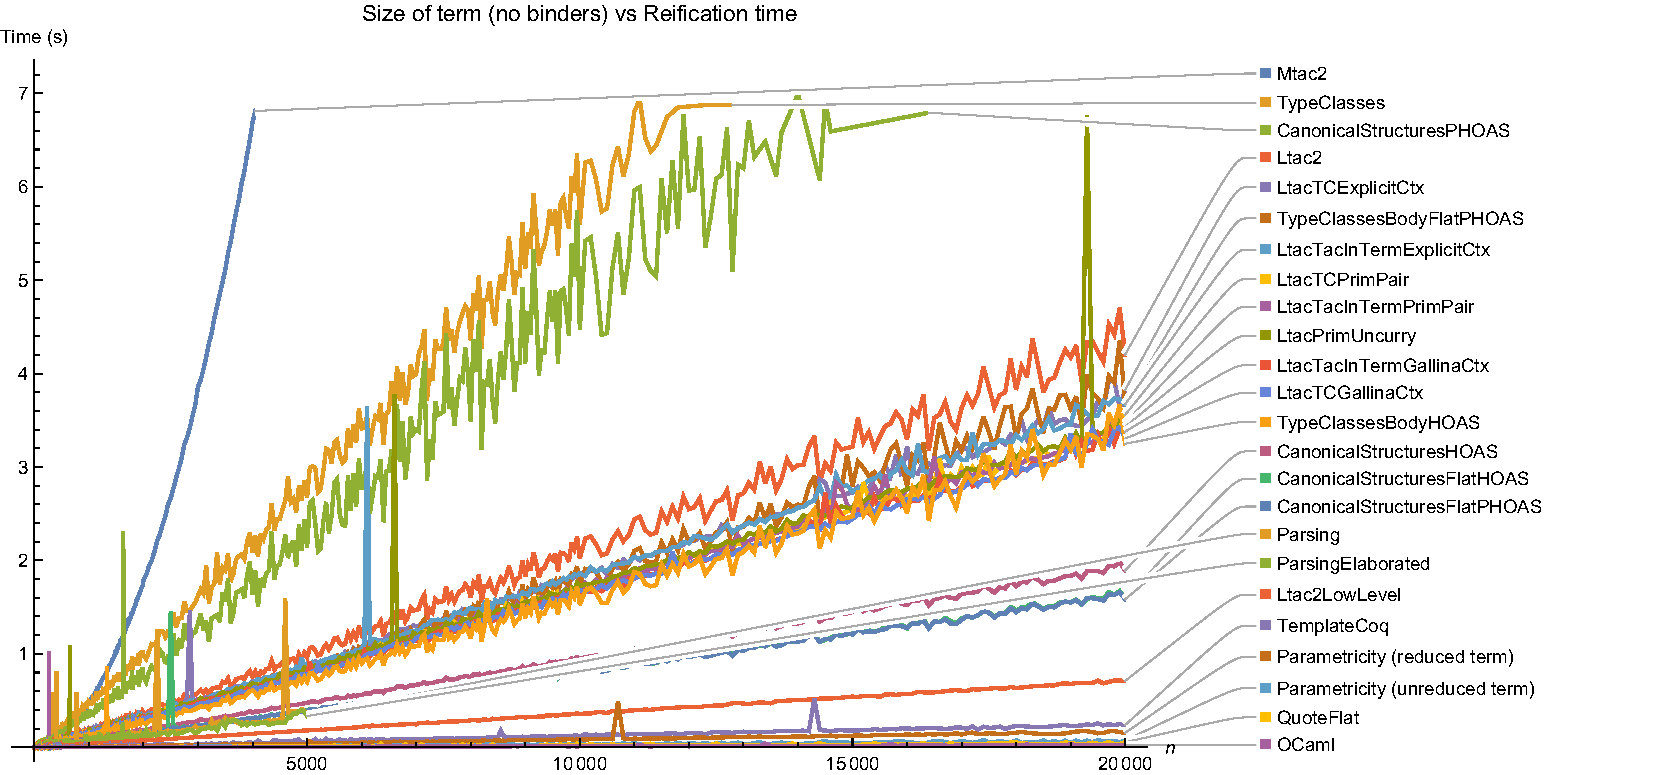
\includegraphics[width=\textwidth]{reification-by-parametricity/actual-reif-no-binders.pdf}
\caption{Performance of Reification without Binders}\label{fig:graph-reif-no-binders}
\end{figure}

Sorted from slowest to fastest, most of the labels in \autoref{fig:graph-reif-no-binders} should be self-explanatory and are found in similarly named \texttt{.v} files in the associated code; we call out a few potentially confusing ones:
\begin{itemize}
  \item
    The ``Parsing'' benchmark is ``reification by copy-paste'': a script generates a \texttt{.v} file with notation for an already-reified term; we benchmark the amount of time it takes to parse and typecheck that term.
    The ``ParsingElaborated'' benchmark is similar, but instead of giving notation for an already-reified term, we give the complete syntax tree, including arguments normally left implicit.
    Note that these benchmarks cut off at around 5000 rather than at around 20\,000, because on large terms, Coq crashes with a stack overflow in parsing.
    %For size reasons, we do not include these \texttt{.v} files in the associated code tarball, but they can be made via the \texttt{parsing-test-files} target, which generates some files in \texttt{Benchmarks/}.
%  \item
%    In \autoref{sec:ltac2-reif} we mention both a naive transcription of \Ltac1 to \Ltac2 and a procedure using low-level primitives in \Ltac2; ``Ltac2'' benchmarks the former, and ``Ltac2LowLevel'' benchmarks the latter.
  \item
    We have four variants starting with ``CanonicalStructures'' here.
    The Flat variants reify to \texttt{@expr nat} rather than to \texttt{forall var, @expr var} and benefit from fewer function binders and application nodes.
    The HOAS variants do not include a case for \letindots\space nodes, while the PHOAS variants do.
    Unlike most other reification methods, there is a significant cost associated with handling more sorts of identifiers in canonical structures.
\end{itemize}

We note that on this benchmark our method is slightly faster than template-coq, which reifies to de Bruijn indices, and slightly slower than the quote plugin in the standard library and the OCaml plugin we wrote by hand.

\subsection{With Binders} \label{sec:perf:binders}

We look at terms of the form \texttt{dlet a$_1$ := 1 * 1 in dlet a$_2$ := a$_1$ * a$_1$ in \ldots\space dlet a$_n$ := a$_{n-1}$ * a$_{n-1}$ in a$_n$}, where $n$ is the size of the term.
The first graph shown here includes all of the reification variants at linear scale, while the next step zooms in on the highest-performance variants at log-log scale.

\begin{figure}[t]
\noindent 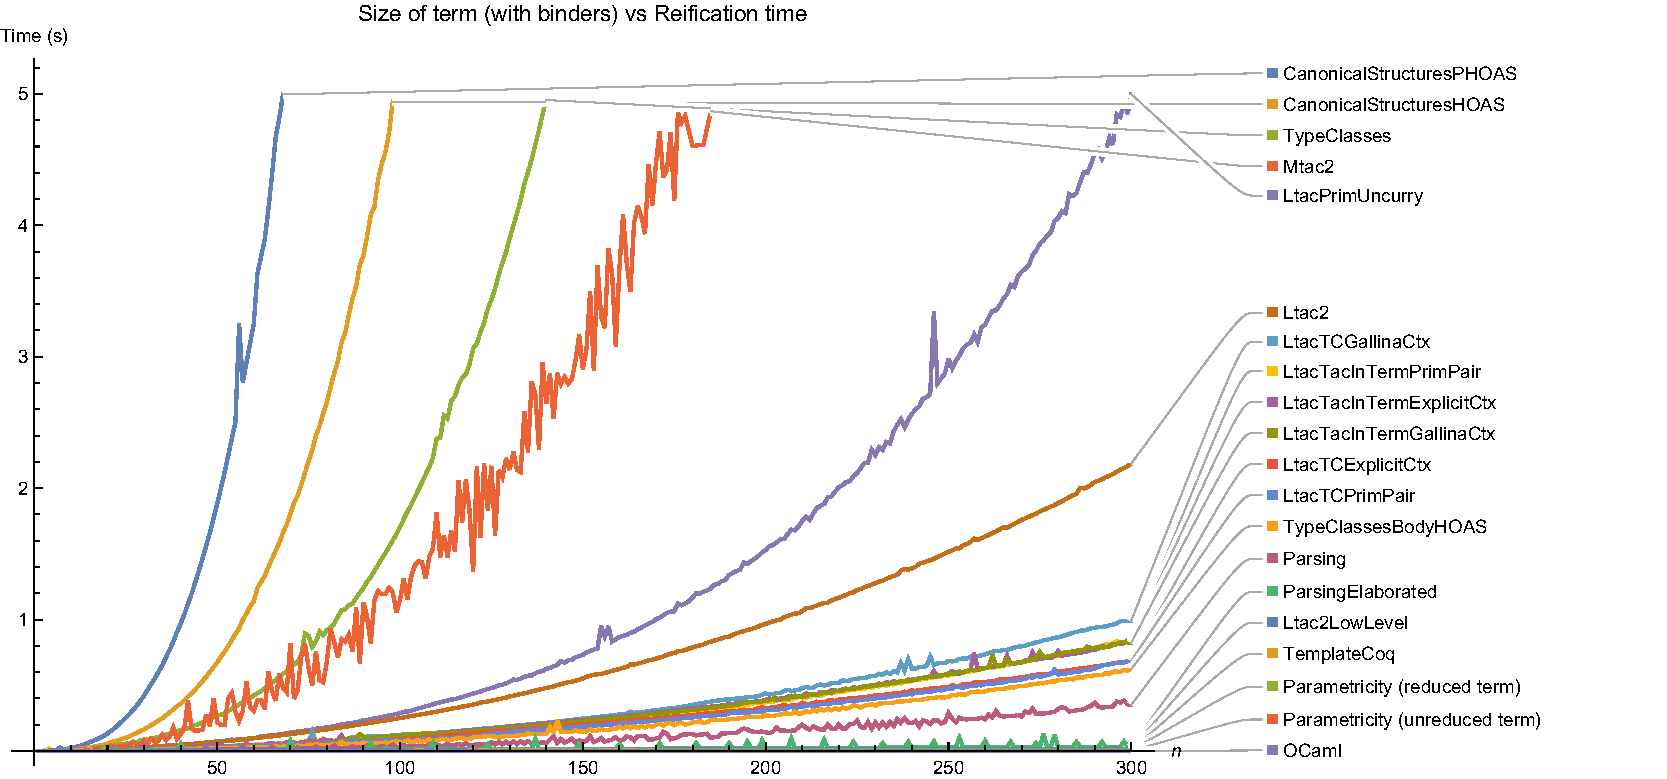
\includegraphics[width=\textwidth]{reification-by-parametricity/actual-reif-with-binders.pdf}

\noindent 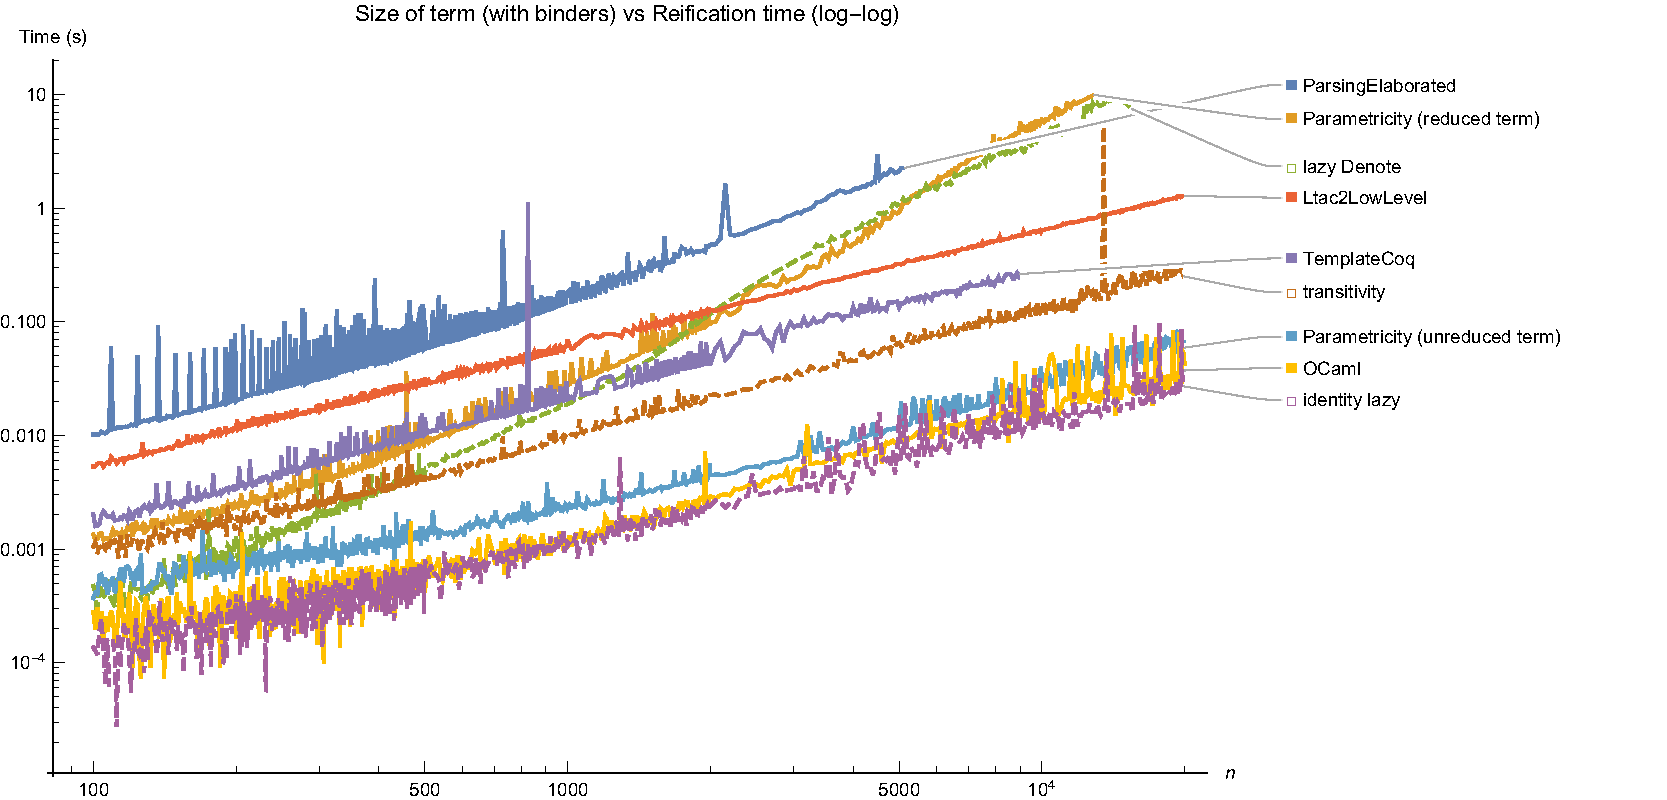
\includegraphics[width=\textwidth]{reification-by-parametricity/actual-reif-with-binders-log-log-subset.pdf}
\caption{Performance of Reification with Binders}\label{fig:reif-binders}
\end{figure}

In addition to reification benchmarks, the graph in \autoref{fig:reif-binders} includes as a reference (1) the time it takes to run \texttt{lazy} reduction on a reified term already in normal form (``identity lazy'') and (2) the time it takes to check that the reified term matches the original native term (``lazy Denote'').
The former is just barely faster than OCaml reification; the latter often takes longer than reification itself.
The line for the template-coq plugin cuts off at around 10\,000 rather than around 20\,000 because at that point template-coq starts crashing with stack overflows.

A nontrivial portion of the cost of ``Parametricity (reduced term)'' seems to be due to the fact that looking up the type of a binder is linear in the number of binders in the context, thus resulting in quadratic behavior of the retyping step that comes after abstraction in the \texttt{pattern} tactic.
In Coq 8.8, this lookup will be $\log n$, and so reification will become even faster~\cite{coq-pr-fast-rel-lookup}.

\section{Future Work, Concluding Remarks} \label{sec:future}

We identify one remaining open question with this method that has the potential of removing the next largest bottleneck in reification: using reduction to show that the reified term is correct.

\begin{wrapfigure}[9]{r}{8cm}
%\vspace{-36pt}
\[
\xymatrix@R=0.5em@C=0em{
    \txt{unreduced term} \ar[d]^{\delta} \\
    \txt{small partially \\ reduced term}
    \ar@<1ex>[ddr]
    \ar@<-1ex>@{--}[rr]
    &&
    \txt{unreduced \\ reified syntax}
    \ar@<-1ex>@{--}[ll]^{???}
    \ar@<1ex>[ddl]
    \\ \\
    &
    \txt{unreduced \\ abstracted term}
    \ar@<1ex>[uul]
    \ar@<1ex>[uur]%^{\rotatebox{40}{\llap{\text{application\hspace*{-2em}}}}}
}
\]
%\vspace{-18pt}
\caption{Completing the commutative triangle}\label{fig:reify-denote-parametricity}
\end{wrapfigure}
Recall our reification procedure and the associated diagram, from \autoref{sec:expanded-reif-diagram}.
We perform $\delta$ on an unreduced term to obtain a small, partially reduced term;
we then perform abstraction to get an abstracted, unreduced term, followed by application to get unreduced reified syntax.
These steps are all fast.
Finally, we perform $\beta\iota$-reduction to get reduced, reified syntax and perform $\beta\iota\delta$ reduction to get back a reduced form of our original term.
These steps are slow, but we must do them if we are to have verified reflective automation.

It would be nice if we could prove this equality without ever reducing our term.
That is, it would be nice if we could have the diagram in \autoref{fig:reify-denote-parametricity}.

The question, then, is how to connect the small partially reduced term with \texttt{denote} applied to the unreduced reified syntax.
That is, letting $F$ denote the unreduced abstracted term, how can we prove, without reducing $F$, that
\[
F\ \mathbb{N}\ \text{Mul}\ \text{O}\ \text{S}\ (\text{@Let\_In }\mathbb{N}\texttt{ }\mathbb{N})
=
\texttt{denote}\ \left(F\ \texttt{expr}\ \texttt{NatMul}\ \texttt{NatO}\ \texttt{NatS}\ \texttt{LetIn}\right)
\]

We hypothesize that a form of internalized parametricity would suffice for proving this lemma.
In particular, we could specialize $F$'s type argument with $\mathbb N \times \texttt{expr}$.
Then we would need a proof that for any function $F$ of type
\[
\forall (T : \texttt{Type}), (T \to T \to T) \to T \to (T \to T) \to (T \to (T \to T) \to T) \to T
\]
and any types $A$ and $B$, and any terms $f_A : A \to A \to A$, $f_B : B \to B\to B$, $a : A$, $b : B$, $g_A : A \to A$, $g_B : B \to B$, $h_A : A \to (A \to A) \to A$, and $h_B : B \to (B \to B) \to B$, using $f\times g$ to denote lifting a pair of functions to a function over pairs:
\begin{align*}
  & \texttt{fst}\ \left(F\ (A \times B)\ (f_A \times f_B)\ (a, b)\ (g_A \times g_B)\ (h_A \times h_B)\right) = F\ A\ f_A\ a\ g_A\ h_A \;\wedge \\
  & \texttt{snd}\ \left(F\ (A \times B)\ (f_A \times f_B)\ (a, b)\ (g_A \times g_B)\ (h_A \times h_B)\right) = F\ B\ f_B\ b\ g_B\ h_B
\end{align*}
This theorem is a sort of parametricity theorem.

Despite this remaining open question, we hope that our performance results make a strong case for our method of reification; it is fast, concise, and robust.
